\documentclass[c,compress]{beamer}
\usetheme{Boadilla}
\usecolortheme{dolphin}
\renewcommand{\baselinestretch}{1.5} 
\usepackage{cite}
\usepackage{amsmath,amssymb,amsfonts}
\usepackage{algorithmic}
\usepackage{graphicx}
\usepackage{diagbox}
\usepackage{array,multirow}
\usepackage{minted}
\usepackage[T1]{fontenc}
\usepackage{booktabs}
% \usepackage{eucal}
\newcommand*{\textcal}[1]{%
  % family qzc: Font TeX Gyre Chorus (package tgchorus)
  % family pzc: Font Zapf Chancery (package chancery)
  \textit{\fontfamily{qzc}\selectfont#1}%
}

\usepackage{hyperref}
\hypersetup{
	pdftitle={JournalClub_AiF},
   colorlinks=false,
   citecolor=blue,
   linkcolor=black,
   urlcolor=blue
}

\usefonttheme{structurebold}
\setbeamercolor{title}{fg=black}
\setbeamercolor{frametitle}{fg=black}
\title{\href{https://arxiv.org/pdf/1905.11481.pdf}{AI Feynman}}
\author{Anil Radhakrishnan}
\institute{University of Illinois}
\date{ML Journal Club, July 9 2020 }
\addtobeamertemplate{navigation symbols}{}{%
    \usebeamerfont{footline}%
    \usebeamercolor[fg]{footline}%
}
\definecolor{blue(pigment)}{rgb}{0.2, 0.2, 0.6}
\def\bsq{\color{blue(pigment)} $\blacksquare$ \color{black}}



\begin{document}

\frame{\titlepage}

% Slide 1
\begin{frame}\frametitle{Motivation} \label{Motiv}
\bsq Finding a symbolic expression that matches data from an unknown function is likely to be NP-hard in principle.\\
\bsq Functions of practical interest often exhibit simplifying properties like symmetries, separability and compositionality.\\
\bsq Physics inspired techniques can be combined with neural networks to develop a multidimensional symbolic regression algorithm
\end{frame} 

% Slide 1
\begin{frame}\frametitle{Introduction} \label{intro}
\bsq Symbolic regression is finding a symbolic expression that matches data from an unknown function\\
\bsq Exponentially large search space makes brute force solutions effectively impossible\\
\bsq Neural networks can be used to discover hidden simplicity to reduce the number of variables
\end{frame} 


\begin{frame}\frametitle{Methods}
\label{Method}
\begin{columns}
 \begin{column}{.69\textwidth}
  \begin{itemize}
    \item Dimensional Analysis
    \item Brute Force
    \item Polynomial fit
    \item {Neural Network
    \begin{itemize}
        \item Check for symmetry
        \item Check for separability
        \item Make 2 variables equal
    \end{itemize}}
    \item Apply unary transformation on the variables
\end{itemize}
 \end{column}

 \begin{column}{.30\textwidth}
  \begin{picture}(2,2)
   \put(0,0){\dashbox{0.2}(2,2)}
  \end{picture}
 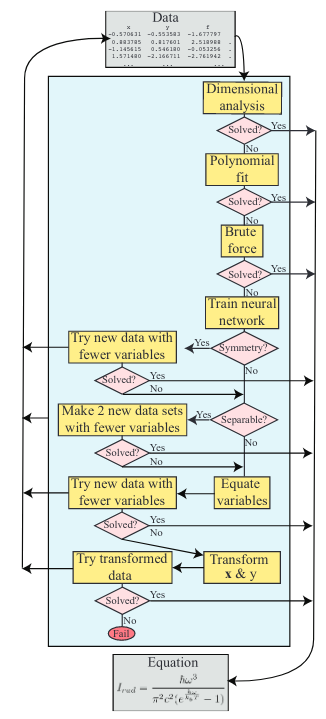
\includegraphics[height=0.8\textheight,keepaspectratio]{algo_scheme.png}
 \end{column}
\end{columns}

\end{frame}


\begin{frame}\frametitle{Dimensional Analysis} \label{DA}

\begin{itemize}
    \item Represent the units of each variable by a six dimensional vector

\begin{table}[]
\centering
\begin{tabular}{@{}lllllll@{}}
\toprule
 Variables & Units & m & s & kg & T & V \\ \midrule
$a,g$ & Acceleration & 1 & -2 & 0 & 0 & 0 \\
$L$  & Angular Momentum & 2 & -1 & 1 & 0 & 0 \\
$k_B$  & Boltzmann constant & 2 & -2 & 1 & -1 & 0 \\
$C$  & Capacitance & 2 & -2 & 1 & 0 & -1 \\ \bottomrule
\end{tabular}
\end{table}
    \item Number of independent variables can be significantly reduced
    \item The null space of the matrix gives the dimensionless variables
\end{itemize}
\end{frame}

\begin{frame}\frametitle{Neural Network -- Check for symmetry}
\label{Method}
\begin{columns}
 \begin{column}{.49\textwidth}
  \begin{itemize}
    \item for a given function $f(x_1, x_2, ...x_n)$ calculates $f(x_1+a, x_2+a,...x_n)$
    \item if equal within precision $f$ depends on $x_1$ and $x_2$ only through their difference
    \item Then $x_1$ and $x_2$ can be replaced by $x_1' \equiv x_1 - x_2 $
\end{itemize}
 \end{column}

 \begin{column}{.49\textwidth}
  \begin{picture}(2,2)
   \put(0,0){\dashbox{0.2}(2,2)}
  \end{picture}
 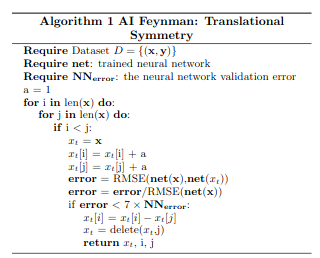
\includegraphics[height=0.5\textheight,keepaspectratio]{trans_sym.png}
 \end{column}
\end{columns}
\end{frame}


\begin{frame}\frametitle{Check for separability}
\label{Method}
\begin{columns}
 \begin{column}{.49\textwidth}
  \begin{itemize}
    \item check if $f(x_1,x_2)$ can be split into $g(x_1)h(x_2)$
    \item if $f(x_1,x_2)=\dfrac{f(x_1,c_2)f(c_1,x_2)}{f(c_1,c_2)}$ within precision, $f$ is multiplicatively separable
    \item similarly for additive separability $f(x_1,x_2) = g(x_1) + h(x_2)$
\end{itemize}
 \end{column}

 \begin{column}{.49\textwidth}
  \begin{picture}(2,2)
   \put(0,0){\dashbox{0.2}(2,2)}
  \end{picture}
 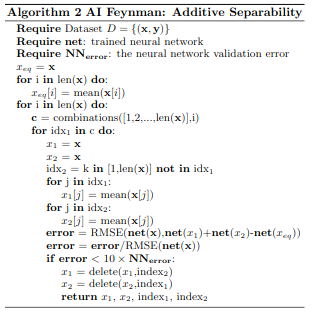
\includegraphics[height=0.5\textheight,keepaspectratio]{add_sep.png}
 \end{column}
\end{columns}
\end{frame}


\begin{frame}\frametitle{Example Procedure}
\label{eg}
\begin{figure}
    \centering
    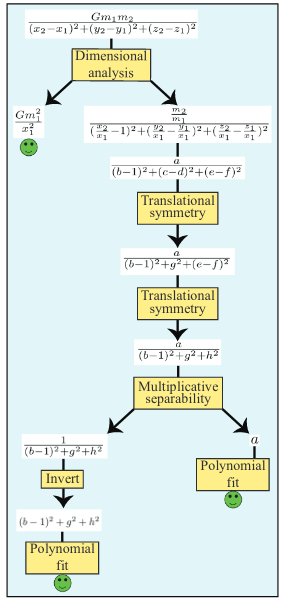
\includegraphics[height=0.8\textheight,keepaspectratio]{example_scheme.png}
\end{figure}
 

\end{frame}

\begin{frame}{Results\\\rule{10.5cm}{0.5pt}} \label{Method}

\bsq Discovered 100 equations from Feynman lectures in Physics with a run time between 10 seconds and 2 hours per equation\\
\bsq Previously state of the art genetic algorithm discovered 71 equation\\
\bsq Adding noise
\begin{itemize}
    \item 95\% of equation solved with Gaussian noise of $\epsilon = 10^{-4}$
    \item 40\% when $\epsilon = 10^{-2}$
\end{itemize}
\bsq The algorithm also works well with reduced data ($\approx 10^2 - 10^5$)
\end{frame}

\begin{frame}{Conclusions\\\rule{10.5cm}{0.5pt}} \label{Conclusions}

\begin{itemize}
    \item New algorithm for symbolic regression using properties of functions of practical interest
    \item Expressions for complicated functions  can be found using dimension analysis and breaking functions using NNs.
    \item Results significantly better than that from genetic algorithms
    \item Good results even with significant noise and less data
\end{itemize}
\end{frame}


\end{document}